\section{Introduction}
The purpose of this chapter is to report the tests that have been done to find the best value of \underline{height} in a Skip List.
Skip List is a probabilistic data structure that allows searching, insertion and deleting operation with time complexity of $O(log n)$.

\section{Testing methodology}
I wrote a bash script\footnote{Included in the repo,the name is \textbf{time\_taker\_ex2.sh}} that runs the program with different values of \underline{height} and saves the output in a file, the range of tested level is between 6 and 50
\newline
\begin{figure}[H]
  \centering
  \begin{minipage}{.45\textwidth}
    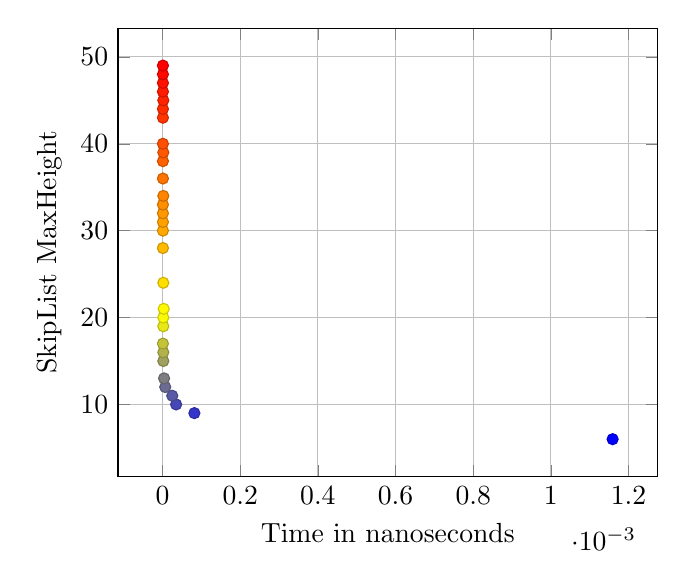
\begin{tikzpicture}
      \begin{axis}[
        ylabel={SkipList MaxHeight},
        xlabel={Time in nanoseconds},
        grid=major,
        legend pos=north west,
      ]
    
      % Add your data points here
      % The 'nan' values indicate that the algorithm did not terminate for those max_height values
      \addplot+[
        scatter,
        only marks,
        error bars/.cd,
        y dir=both,
        y explicit,
        error bar style={line width=1pt},
      ] table[
        x index=0,  % Use the first column as x
        y index=1,  % Use the second column as y
        col sep=comma,
      ] {
    x, y
    nan, 2
    nan, 3
    nan, 4
    nan, 5
    0.001159, 6 
    0.000082, 9 
    0.000035, 10 
    0.000025, 11 
    0.000007, 12 
    0.000004, 13 
    0.000002, 15 
    0.000002, 16 
    0.000001, 17 
    0.000002, 19 
    0.000002, 20 
    0.000003, 21 
    0.000002, 24 
    0.000001, 28 
    0.000001, 30 
    0.000001, 31 
    0.000001, 32 
    0.000001, 33 
    0.000002, 34 
    0.000001, 36 
    0.000001, 38 
    0.000002, 39 
    0.000001, 40 
    0.000001, 43 
    0.000001, 44 
    0.000002, 45 
    0.000001, 46 
    0.000001, 47 
    0.000001, 48 
    0.000001, 49  
      };
    
      \end{axis}
    \end{tikzpicture}
    \caption{Graph 1: SkipList MaxHeight vs. Time}
  \end{minipage}%
  \hfill
  \hspace{0.15\textwidth}
  \begin{minipage}{.45\textwidth}
    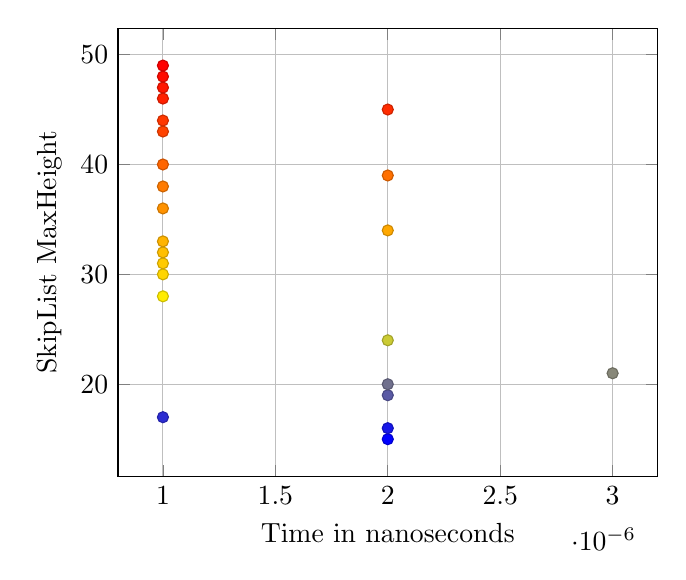
\begin{tikzpicture}
      \begin{axis}[
        ylabel={SkipList MaxHeight},
        xlabel={Time in nanoseconds},
        grid=major,
        legend pos=north west,
      ]
    
      % Add data for the second graph here
      \addplot+[
        scatter,
        only marks,
        error bars/.cd,
        y dir=both,
        y explicit,
        error bar style={line width=1pt},
      ] table[
        x index=0,
        y index=1,
        col sep=comma,
      ] {
    0.000002, 15 
    0.000002, 16 
    0.000001, 17 
    0.000002, 19 
    0.000002, 20 
    0.000003, 21 
    0.000002, 24 
    0.000001, 28 
    0.000001, 30 
    0.000001, 31 
    0.000001, 32 
    0.000001, 33 
    0.000002, 34 
    0.000001, 36 
    0.000001, 38 
    0.000002, 39 
    0.000001, 40 
    0.000001, 43 
    0.000001, 44 
    0.000002, 45 
    0.000001, 46 
    0.000001, 47 
    0.000001, 48 
    0.000001, 49 
      };
    
      \end{axis}
    \end{tikzpicture}
    \caption{Graph 2: SkipList MaxHeight vs. Time (Focused)}
  \end{minipage}
\end{figure}



\newline
Range from 1 to 5 is omitted because the algorithm did not terminate for those values
\footnote{all test are done on a Lenovo Thinkpad x390 yoga with an Intel Core i7-8565U CPU and 16GB of RAM, with Arch Linux installed as only OS}


\section{Conclusion based on the analysis}
Looking the graph the best values is between 15 and 20, because this range is the good balance between the time used to search the words in the skip list and the memory used. 

\section{Knwon Issues}
Sometimes the main program gives a segmentation fault error caused by the \textbf{fgets()},used to read the phrase to correct, on 50 run the program gave segmentatin fault 7 times.